\documentclass[a4paper]{article}

\usepackage{INTERSPEECH_v2}
\usepackage{color}
\usepackage{hyperref}
\usepackage{subcaption}

\DeclareMathOperator*{\minp}{min^\prime}

\title{Graph Neural Networks with Efficient Tensor Operations in CUDA/GPU and GraphFlow Deep Learning Framework in C++ for Quantum Chemistry}
% and GraphFlow Deep Learning Framework in C++ for Quantum Chemistry}
\name{Hy Truong Son, Chris Jones}
\address{Department of Computer Science, The University of Chicago}
\email{hytruongson@uchicago.edu, csj@uchicago.edu}

\begin{document}
\pagestyle{headings}

\maketitle
% 
\begin{abstract}
In this paper, we propose Covariant Compositional Networks (CCNs), state-of-the-art generalized convolution graph neural networks for learning graphs. By applying higher-order graph representations and tensor contraction operations that are permutation-invariant with respect to the set of vertices, CCNs address the representation limitation of all existing neural networks for learning graphs. To efficiently implement graph neural networks, which require expensive tensor operations, we designed our custom deep learning framework in C++, GraphFlow, that supports dynamic computation graphs, automatic and symbolic differentiation, as well as tensor/matrix implementation in CUDA to speed up computation with GPUs. For an application of graph neural networks in quantum chemistry and molecular dynamics, we investigate the efficiency of CCNs in simulating Density Functional Theory (DFT) which is the most successful and widely used (yet computationally expensive) approach to computing the electronic structure of matter. We obtain a very promising result and outperform other state-of-the-art models on the Harvard Clean Energy Project molecular dataset. \\
\end{abstract}
\noindent\textbf{Index Terms}: graph neural network, message passing, representation theory, density functional theory, molecular dynamics

\section{Introduction}

In the field of machine learning, standard objects such as vectors, matrices, and tensors have been carefully studied and successfully applied to various areas including computer vision, natural language processing, speech recognition, etc. However, none of these standard objects are effecitve at capturing the structure of molecules, social networks, or the World Wide Web, all of which have a rich underlying graph structure. Thus there is a need for native graph representation and extensions of Support Vector Machine and Convolution Neural Networks to graphs. \\ \\
To represent graphs in general and molecules specifically, a proposed model must be \textit{permutation-invariant} and \textit{rotation-invariant}. In addition, to apply kernel methods to graphs, a proposed kernel must be \textit{positive semi-definite}. Many graph kernels and graph similarity functions have been introduced by researchers. Among them, one of the most successful and efficient is the Weisfeiler-Lehman graph kernel, which aims to build a multi-level, hierarchical representation of a graph \cite{Nino}. However, a limitation of kernel methods is their quadratic space usage and quadratic time complexity. In this paper, we address this drawback by proposing Dictionary Weisfeiler-Lehman graph features in combination with Morgan circular fingerprints. The common idea in the family of Weisfeiler-Lehman graph kernel is to hash the sub-structures of a graph. Extending this idea, we arrive at the simplest form of graph neural networks in which the \textit{fixed} hashing function is replaced by a \textit{learnable} one such as a non-linearity mapping. The details of this idea are given in Section 3.1. We detail the graph neural network baselines, such as Neural Graph Fingerprint \cite{Duvenaud} and Learning Convolutional Neural Networks \cite{Niepert}, in Section 3.2. In the context of graphs, the sub-structures can be viewed as a set of vertex feature vectors. We utilize the convolution operation to introduce higher-order representations for each vertex, from zero-order as a vector to first-order as a matrix and second-order as a 3-order tensor; this is described in Section 3.3. Also in this section, we introduce the notions of tensor contractions and tensor products to keep the size of all tensors manageable. Our generalized convolution graph neural network as described in the preceding paragraph is named a Covariant Compositional Network. \\ \\
Current Deep Learning frameworks including TensorFlow \cite{Google-Research}, PyTorch \cite{PyTorch}, Mxnet \cite{Mxnet}, Theano \cite{Theano} show limitations for constructing dynamic computation graphs along with specialized tensor operations. There is a need for a flexible programming framework for graph neural networks addressing both these drawbacks. With this motivation, we designed our deep learning framework in C++, GraphFlow, for our long-term machine learning research. All of our experiments have been implemented efficiently within GraphFlow. In addition, GraphFlow is parallelized with CPU/GPU multi-threading. Implementation of GraphFlow is described in Chapter 4. We carefully evaluate the performance improvements of GraphFlow before and after parallelization in various experiments, from testing tensor/matrix operations to training on a small molecular dataset. The increased efficiency from parallelization allows for deeper networks to be trained in a reasonable timeframe; the resulting performance gain is significant. These analyses are given in Chapter 5. Finally, we apply our methods to the Harvard Clean Energy Project (HCEP) molecular dataset \cite{Johannes}. The visualizations, experiments and empirical results from this experiment are detailed in Chapter 5. Chapter 6 concludes and presents future research directions.

\begin{figure}[h]
\caption{Two molecules with adjacency matrices in HCEP }
\label{fig:molecules}
\centering
\begin{subfigure}[h]{0.5\columnwidth}
	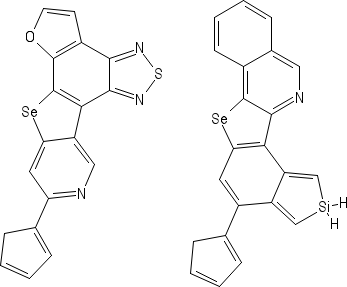
\includegraphics[width=\textwidth]{sketcher2}
\end{subfigure}\\
\begin{subfigure}[h]{0.3\columnwidth}
	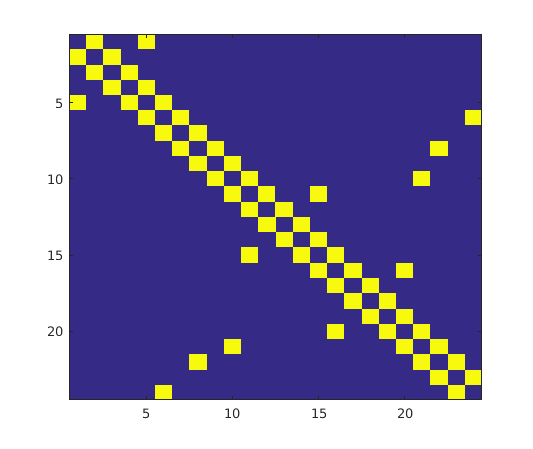
\includegraphics[width=\textwidth]{adjacency1}
     \caption{C$_{18}$H$_9$N$_3$OSSe}
\end{subfigure}
\begin{subfigure}[h]{0.3\columnwidth}
	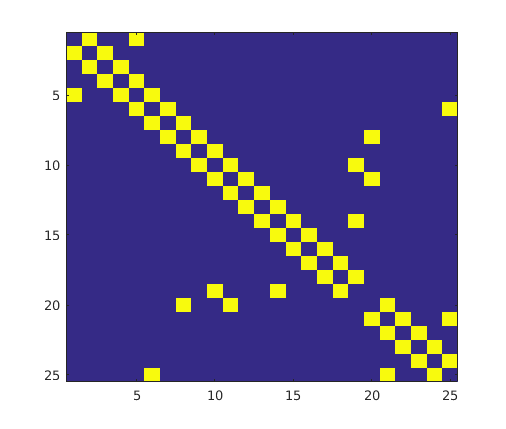
\includegraphics[width=\textwidth]{adjacency2}
	\caption{C$_{22}$H$_{15}$NSeSi}
\end{subfigure}
\end{figure}

\section{Related Work}

The notion of graph kernel was first introduced by Kondor and Lafferty in \cite{Risi}. Borgwardt and colleagues proposed the state-of-the-art Weisfeiler-Lehman graph kernel, based on the famous Weisfeiler-Lehman test for graph isomorphism \cite{Nino}. N. M. Kriege, P. L. Giscard and R. C. Wilson applied the Hungarian matching algorithm to define a more robust Weisfeiler-Lehman graph kernel \cite{Nils}. The convolution operation on graphs from Section 3.3, as well as graph neural networks for learning molecular fingerprints, are mentioned by other authors \cite{Steven}, \cite{Duvenaud}, and \cite{Thomas}, without implementation of an efficient tensor contraction algorithm.

\section{Methods}

\subsection{Graph Kernel}

\subsubsection{Positive Semi-definite Kernel}

Say we're given two undirected graphs $G_1 = (V_1, E_1)$ and $G_2 = (V_2, E_2)$. Further assume each vertex is associated with a feature vector $f: V \rightarrow \Omega$. A \textit{positive semi-definite} graph kernel between $G_1$ and $G_2$ is defined as:
$$\mathcal{K}_{graph}(G_1, G_2) = \frac{1}{|V_1|} \cdot \frac{1}{|V_2|} \cdot \sum\limits_{v_1 \in V_1} \sum\limits_{v_2 \in V_2} k_{base}(f(v_1), f(v_2))$$
where $k_{base}$ is any base kernel and can be:
\begin{itemize}
	\item Linear: $k_{base}(x, y) = \langle x, y \rangle_{norm} = x^Ty / (\|x\| \cdot \|y\|)$
	\item Quadratic: $k_{base}(x, y) = (\langle x, y \rangle_{norm} + q)^2$
	\item RBF: $k_{base}(x, y) = \exp(-\gamma \|x - y\|^2)$
\end{itemize}

\subsubsection{Weisfeiler-Lehman Graph Features}

We combine the Weisfeiler-Lehman graph kernel \cite{Nino} and Morgan circular fingerprints into the Dictionary Weisfeiler-Lehman graph feature algorithm. To capture the substructures of a graph, we define a Weisfeiler-Lehman subtree at level $l$ rooted at a vertex $v$ to be the shortest-path subtree that includes all vertices reachable from $v$ by a path of length at most $2^l$. Each subtree is represented by a multiset of vertex labels. We build the Weisfeiler-Lehman dictionary by finding all subtree representations of every graph in the dataset. The graph feature or fingerprint is a frequency vector in which each component corresponds to the frequency of a particular dictionary element. \\ \\
Formally, we have a set of $N$ graphs $\mathcal{G} = \{G^{(1)}, .., G^{(N)}\}$ where $G^{(i)} = (V^{(i)}, E^{(i)})$ $(1 \leq i \leq N)$. Let $f^G: V \rightarrow \Omega$ be the initial feature vector for each vertex of graph $G = (V, E)$. Let $S^G_k(v)$ be the set of vectors for vertex $v \in V$ of graph $G$ at Weisfeiler-Lehman level $k$. \\ \\
\textbf{function} Dictionary Weisfeiler-Lehman \\
01. \ \ \ \ Universal dictionary: $\mathcal{D} \leftarrow \emptyset$ \\
02. \ \ \ \ for $i = 1 \rightarrow N$: \\
03. \ \ \ \ \ \ \ \ \textit{Initialize the WL level 0} \\
04. \ \ \ \ \ \ \ \ for each $v \in V^{(i)}$: \\
05. \ \ \ \ \ \ \ \ \ \ \ \ $S^{G^{(i)}}_0(v) \leftarrow \{f^{G^{(i)}}(v)\}$ \\
06. \ \ \ \ \ \ \ \ \ \ \ \ $\mathcal{D} \leftarrow \mathcal{D} \cup \{S^{G^{(i)}}_0(v)\}$ \\
07. \ \ \ \ \ \ \ \ end for \\
08. \ \ \ \ \ \ \ \ \textit{Build the WL level} $1$, $2$, .., $K$ \\
09. \ \ \ \ \ \ \ \ for $k = 1 \rightarrow K$: \\
10. \ \ \ \ \ \ \ \ \ \ \ \ for each $v \in V^{(i)}$: \\
11. \ \ \ \ \ \ \ \ \ \ \ \ \ \ \ \ $S^{G^{(i)}}_k(v) \leftarrow S^{G^{(i)}}_{k - 1}(v)$ \\
12. \ \ \ \ \ \ \ \ \ \ \ \ \ \ \ \ for each $(u, v) \in E^{(i)}$: \\
13. \ \ \ \ \ \ \ \ \ \ \ \ \ \ \ \ \ \ \ \ $S^{G^{(i)}}_k(v) \leftarrow S^{G^{(i)}}_k(v) \cup S^{G^{(i)}}_{k - 1}(u)$ \\
14. \ \ \ \ \ \ \ \ \ \ \ \ \ \ \ \ end for \\
15. \ \ \ \ \ \ \ \ \ \ \ \ \ \ \ \ $\mathcal{D} \leftarrow \mathcal{D} \cup \{S^{G^{(i)}}_k(v)\}$ \\
16. \ \ \ \ \ \ \ \ \ \ \ \ end for \\
17. \ \ \ \ \ \ \ \ end for \\
18. \ \ \ \ end for \\
19. \ \ \ \ $\mathcal{S} \leftarrow \{S^{G^{(1)}}_0, .., S^{G^{(N)}}_0, .., S^{G^{(1)}}_K, .., S^{G^{(N)}}_K\}$ \\
20. \ \ \ \ \textbf{return} $\mathcal{D}$, $\mathcal{S}$ \\
\textbf{end function}

\subsubsection{Histogram-Alignment Graph Features}

The optimal-assignment Weisfeiler-Lehman graph kernel \cite{Nils} computes the original Weisfeiler-Lehman graph kernel, then applies the Hungarian matching algorithm for bipartite graphs to find the optimal matching between the two sets of vertex feature vectors of the two graphs. One drawback of this approach is the time complexity of the matching algorithm, which is polynomial but $O(n^5)$. To address this problem, we construct a multi-level histogram of frequencies as the fingerprint for each graph, and compare histograms directly. This method is known as \textit{Histogram-alignment Weisfeiler-Lehman graph features}. 

\subsection{Graph Neural Networks}

In this section, we discuss the two state-of-the-art graph neural networks that are our baseline models: Neural Graph Fingerprint (NGF) proposed by Duvenaud et al \cite{Duvenaud}, and Learning Convolutional Neural Networks (LCNN) proposed by Niepert et al \cite{Niepert}. However, these two models have their own drawbacks:
\begin{itemize}
	\item NGF is limited in representation power since each vertex is only represented by a multi-channel vector (and each channel is represented by only a single scalar). In our terminology we classify this type of representation as zero-order. To empower the vertex representation, we introduce first-order and second-order representations in which each channel is representated by a vector and a matrix, and consequently the vertex representations are a matrix and 3-order tensor, respectively.
	\item LCNN is not permutation invariant because it uses the Weisfeiler-Lehman algorithm to rank the vertices into a particular ordering (note that finding an optimal ordering of the set of vertices is an NP-hard problem). This means LCNN is not invariant under a permutation of the vertices. To address this issue, we apply tensor contraction and tensor product operations over higher-order representations of vertices in a way such that the resulting features are perfectly equivariant.
\end{itemize}

\subsubsection{Neural Graph Fingerprint \cite{Duvenaud}}

In this section we describe the NGF model. First of all, we define a simple message passing scheme. Fix an input graph $G = (V, E, A)$, where $V$ is the set of vertices, $E$ is the set of edges and matrix $A \in \{0, 1\}^{|V| \times |V|}$ is the corresponding adjacency matrix. The goal is to learn an unknown class of functions parameterized by $\{W_1, .., W_T, u\}$ under the following generative model:
\begin{enumerate}
    \item The inputs are vectors $f(v) \in \Re^d$ for each vertex $v \in V$. We call the vector embedding $f$ the multi-dimensional vertex label function.
    \item We assume some learnable weight matrix $W_i \in \Re^{d \times d}$ associated with level $i$ of the neural network. For each of $T$ levels, we update the vector stored at vertex $v$ using $W_i$.
    \item Finally, we assume some learnable weight vector $u \in \Re^d$. We add up the iterated vertex labels and dot product the result with $u$. This can be thought of as a linear regression on top of the graph neural network.
\end{enumerate}
More formally, we define the $T$-iteration label propagation algorithm on graph $G$. Let $h_t(v) \in \Re^d$ be the vertex embedding of vertex $v$ at iteration $t \in \{0, \dots, T\}$. At $t = 0$, we initialize $h_0(v) = f(v)$. At $t \in \{1, .., T\}$, we update $h_{t-1}$ to $h_t$ at a vertex $v$ using the values on $v$'s neighbors:
\begin{equation}
h_t(v) = h_{t - 1}(v) + \frac{1}{|\mathcal{N}(v)|}\sum\limits_{w \in \mathcal{N}(v)} h_{t - 1}(w)
\end{equation}
where $\mathcal{N}(v) = \{w \in V | (v, w) \in E\}$ denotes the set of adjacent vertices to $v$. We can write the label propagation algorithm in a matrix form. Let $H_t \in \Re^{|V| \times d}$ denote the vertex embedding matrix in which the $v$-th row of $H_t$ is the embedding of vertex $v$ at iteration $t$. Equation $(1)$ is equivalent to:
\begin{equation}
H_t = (I_{|V|} + D^{-1} \cdot A) \cdot H_{t - 1}
\end{equation}
where $I_{|V|}$ is the identity matrix of size $|V| \times |V|$ and $D$ is the diagonal matrix with entries equal to the vertex degrees. Note that it is also common to define another label propagation algorithm via the normalized graph Laplacian \cite{Thomas}:
\begin{equation}
H_t = (I_{|V|} - D^{-1/2}AD^{-1/2}) \cdot H_{t - 1}
\end{equation}
From the label propagation algorithms, we build the simplest form of graph neural networks \cite{Steven, Duvenaud, Thomas}. Suppose that iteration $t$ is associated with a learnable matrix $W_t \in \Re^{d \times d}$ and a component-wise nonlinearity function $\sigma$; in our case $\sigma$ is the sigmoid function. We imagine that each iteration now becomes a layer of the graph neural network. We assume that each graph $G$ has input labels $f$ and a learning target $\mathcal{L}_G \in \Re$. The forward pass of the graph neural network (GNN) is described by the following algorithm: \\ \\
\textbf{function} Forward($G = (V, E, A)$, $T \in \mathbb{N}$) \\
01. \ \ \ \ Initialize $W_0, W_1, .., W_T \in \Re^{d \times d}$ \\
02. \ \ \ \ Layer $0$: $L_0 = \sigma(H_0 \cdot W_0)$ \\
03. \ \ \ \ Layer $t \in \{1, .., T\}$: $L_t = \sigma(H_t \cdot W_t)$ \\
04. \ \ \ \ Compute the graph feature: $f_G = \sum_{v \in V} L_T(v) \in \Re^d$ \\
05. \ \ \ \ Linear regression on layer $T + 1$ \\
06. \ \ \ \ Minimize: $\|\langle u, f_G \rangle - \mathcal{L}_G\|_2^2$ where $u \in \Re^d$ is learnable \\
\textbf{end function} \\ \\
Learnable matrices $W_i$ and learnable vector $u$ are optimized by the back-propagation algorithm as used when training a conventional multi-layer feed-forward neural network. \\ \\
To build on the Neural Graph Fingerprint, we can also introduce quadratic and cubic aggregation rules. These can be considered a special case of our general model of tensor contractions to be introduced in Section 3.3. In detail, the linear aggregation rule can be defined as the summation of feature vectors in a neighborhood $\mathcal{N}(v)$ of vertex $v$ at level $l - 1$. This yields a permutation invariant representation of vertex $v$ at level $l$:
$$\phi_l^{linear}(v) = \sum\limits_{w \in \mathcal{N}(v)} h_{l - 1}(w)$$
where $\phi_l^{linear}(v) \in \Re^d$ and $h_{l - 1}(w) \in \Re^d$ are zero-order representations such that each of $d$ channels is represented by a single scalar. Extending this we formulate the quadratic aggregation rule, $\phi_l^{quadratic}(v)$:
$$\phi_l^{quadratic}(v) = diag \bigg(\sum\limits_{u \in \mathcal{N}(v)} \sum\limits_{w \in \mathcal{N}(v)} h_{l - 1}(u) h_{l - 1}(w)^T \bigg)$$
where $h_{l - 1}(u) h_{l - 1}(w)^T \in \Re^{d \times d}$ is the outer-product of the level $(l - 1)$-th representation of vertices $u$ and $w$ in the neighborhood $\mathcal{N}(v)$. Again $\phi_l^{quadratic}(v) \in \Re^d$ is still zero-order. Finally, we extend to the cubic aggregation rule for $\phi_l^{cubic}(v)$:
$$\phi_l^{cubic}(v) = diag \bigg( \sum\limits_{u, w, t \in \mathcal{N}(v)} h_{l - 1}(u) \otimes h_{l - 1}(w) \otimes h_{l - 1}(t) \bigg)$$
where $h_{l - 1}(u) \otimes h_{l - 1}(w) \otimes h_{l - 1}(t) \in \Re^{d \times d \times d}$ is the tensor product of three rank-$1$ vectors, and we obtain the zero-order $\phi_l^{cubic}(v) \in \Re^d$ by taking the diagonal of the resulting $3$-order tensor. \\ \\
Moreover, it is slightly unnatural to limit the iteration to only the set of adjacent vertices $\mathcal{N}(v)$  of $v$. Another way to extend $\mathcal{N}(v)$ is to use different neighborhoods at different levels or layers of the network, for example:
\begin{itemize}
	\item At level $l = 0$: $\mathcal{N}_0(v) = \{v\}$
	\item At level $l > 0$: 
	$$\mathcal{N}_l(v) = \mathcal{N}_{l - 1}(v) \cup \bigcup_{w \in B(v, 1)} \mathcal{N}_{l - 1}(w)$$
	where $B(v, 1)$ denotes the set of vertices are at distance $1$ from the center $v$.
\end{itemize}
In Section 3.3, we will discuss further this hierarchical extension of neighborhoods captured in the definition of a receptive field.

\subsubsection{Learning Convolutional Neural Networks \cite{Niepert}}

The idea of LCNNs can be summarized as \textit{flattening} a graph into a fixed-size sequence. Suppose that the maximum number of vertices over the entire dataset is $N$. Consider an input graph $G = (V, E)$. If $|V| < N$ then we add $N - |V|$ \textit{dummy vertices} into $V$ to ensure every graph in the dataset has the same number of vertices. For each vertex $v \in V$, LCNN fixes the size of its neighborhood $\Omega(v)$ as $K$. In the case $|\Omega(v)| < K$, again we add $K - |\Omega(v)|$ dummy vertices into $\Omega(v)$ to ensure that every neighborhood of every vertex has exactly the same number of vertices. Let $d: V \times V \rightarrow \{0, .., |V| - 1\}$ denote the shortest-path distance between any pair of vertices in $G$. Let $\sigma: V \rightarrow \Re$ denote the hashing function obtained via the Weisfeiler-Lehman graph isomorphism test. Based on $\sigma$, we can obtain a sub-optimal ranking of vertices. The neighborhood $\Omega(v)$ of vertex $v$ is constructed by the following algorithm: \\ \\
\textbf{function} Contruct-Neighbor \ ($v \in V$) \\
01. \ \ \ \ $\Omega(v) \leftarrow \emptyset$ \\
02. \ \ \ \ for each distance $l \in {0, .., |V| - 1}$: \\
03. \ \ \ \ \ \ \ \ for each vertex $w \in V$: \\
04. \ \ \ \ \ \ \ \ \ \ \ \ if $d(v, w) = l$: \\
05. \ \ \ \ \ \ \ \ \ \ \ \ \ \ \ \ $\Omega(v) \leftarrow \Omega(v) \cup \{w\}$ \\
06. \ \ \ \ \ \ \ \ \ \ \ \ end if \\
07. \ \ \ \ \ \ \ \ end for \\
08. \ \ \ \ \ \ \ \ if $|\Omega(v)| \ge K$: \\
09. \ \ \ \ \ \ \ \ \ \ \ \ break \\
10. \ \ \ \ \ \ \ \ end if \\
11. \ \ \ \ end for \\
12. \ \ \ \ if $|\Omega(v)| < K$: \\
13. \ \ \ \ \ \ \ \ Add $K - |\Omega(v)|$ dummy vertices into $\Omega(v)$ \\
14. \ \ \ \ end if \\
15. \ \ \ \ Suppose $\Omega(v) = \{v_1, .., v_K\}$ \\
16. \ \ \ \ Sort $\Omega(v) \leftarrow \{v_{i_1}, .., v_{i_K}\}$ such that $\sigma(v_{i_t}) < \sigma(v_{i_{t + 1}})$ \\
17. \ \ \ \ Return $\Omega(v)$ \\
\textbf{end function} \\ \\
We also have an algorithm to flatten the input graph $G$ as follows into a sequence of $N \times K$ vertices: \\ \\
\textbf{function} Flatten-Graph ($G = (V, E)$) \\
01. \ \ \ \ Suppose that $V = \{v_1, .., v_{|V|}\}$ \\
02. \ \ \ \ Sort $\bar{V} \leftarrow \{v_{i_1}, .., v_{i_{|V|}}\}$ such that $\sigma(v_{i_t}) < \sigma(v_{i_{t + 1}})$ \\
03. \ \ \ \ Output sequence $S \leftarrow \emptyset$ \\
04. \ \ \ \ for each $v \in \bar{V}$: \\
05. \ \ \ \ \ \ \ \ Add $\Omega(v)$ at the end of $S$ \\
06. \ \ \ \ end for \\
07. \ \ \ \ return $S$ \\
\textbf{end function} \\ \\
Suppose that each vertex is associated with a fixed-size input feature vector of $L$ channels. By the Flatten-Graph algorithm, we can produce a feature matrix of size $L \times (NK)$. We can apply the standard convolution operation as a 1-dimensional Convolutional Neural Network on the columns of this matrix. On top of LCNN is a fully-connected layer for regression tasks or classification tasks.  

\subsection{Covariant Compositional Networks}

\subsubsection{Generic Algorithm}

Covariant Compositional Networks are designed to have a hierarchical and multi-scale structure with multiple levels or layers that capture the structure of the input graph, from local scale to global scale. Furthermore, the data carried at the various levels of the network is built in such a way that representations of higher levels are built based on representations of lower levels, and critically all representations have permutation and rotation invariance. First of all, we recursively define a generalization of the neighborhood of a vertex, the hierarchical receptive field $\Omega_l(v)$ of a vertex $v$ at level $l$:
\begin{itemize}
	\item $\Omega_0(v) = \{v\}$
	\item $\Omega_l(v) = \Omega_{l - 1}(v) \cup \bigcup_{w \in B(v, 1)} \Omega_{l - 1}(w)$
\end{itemize} 
The receptive field should be thought of as the set of vertices centered at $v$, with the parameter $l$ describing how ``deep" we look out from $v$. The data for $v$ at level $l$ of the CCN will be aggregated from $\Omega_l(v)$ via a generalized message passing scheme. Based on the definition of $\Omega_l(v)$, we generalize the vertex represetation $f_l(v)$ to higher-order representations. The zero-order representation limits $f_l(v)$ to be a vector of $d$ channels as discussed in Section 3.2. \\ \\
The first-order representation allows each of the $d$ channels of $f_l(v)$ to be represented by a vector of size $|\Omega_l(v)|$ in which each element of this vector corresponds to a vertex in the receptive field $\Omega_l(v)$. Thus in the first-order representation, $f_l(v) \in \Re^{|\Omega_l(v)| \times d}$ where each row of $f_l(v)$ is a zero-order representation of $d$ channels of a vertex in $\Omega_{l}(v)$ at level $l - 1$. \\ \\
More generally, the second-order representation allows each channel of $d$ channels of $f_l(v)$ to be represented by a symmetric matrix of size $|\Omega_l(v)| \times |\Omega_l(v)|$. Thus, $f_l(v) \in |\Omega_l(v)| \times |\Omega_l(v)| \times d$ is a 3-order tensor. \\ \\
The first-order aggregation rule can be defined as follows:
$$\phi_l^{first}(v) = \sum\limits_{w \in \Omega_l(v)} X_l(v, w) f_{l - 1}(w)$$
where $f_{l - 1}(w) \in \Re^{|\Omega_{l - 1}(w)| \times d}$ for each $w \in \Omega_l(v)$, and $X_l(v, w) \in \{0, 1\}^{|\Omega_l(v)| \times |\Omega_{l - 1}(w)|}$ is a permutation matrix defined as follows:
\begin{itemize}
	\item $X_l(v, w)_{ij} = 1$: if $\Omega_l(v)_i = \Omega_{l - 1}(w)_j$
	\item $X_l(v, w)_{ij} = 0$: otherwise
\end{itemize}
This permutation matrix arranges vertices in $\Omega_{l - 1}(w)$ into the correct position in $\Omega_l(v)$. Remark that $\Omega_{l - 1}(w) \subseteq \Omega_l(v)$. By definition, the first-order aggregation rule gives us the first-order representation $\phi_l^{first}(v) \in \Re^{|\Omega_l(v)| \times d}$. The second-order aggregation rule can be defined as follows:
$$\phi_l^{second}(v) = \sum\limits_{w \in \Omega_l(v)} X_l(v, w) \otimes f_{l - 1}(w) \otimes X_l(v, w)^T$$
where $f_{l - 1}(w) \in \Re^{|\Omega_{l - 1}(w)| \times |\Omega_{l - 1}(w)| \times d}$ for each $w$, operatior $\otimes$ is the broad-casting matrix-tensor multiplication, and $X_l(v, w) \in \Re^{|\Omega_l(v)| \times |\Omega_{l - 1}(w)|}$ is the permutation matrix defined as above. The second-order aggregation rule gives us the second-order representation $\phi_l^{second}(v) \in \Re^{|\Omega_l(v)| \times |\Omega_l(v)| \times d}$. \\ \\
The generic learning rule can be expressed as:
$$f_l(v) = \sigma \big( b_l + W_l \otimes \phi_l(v) \big)$$
where $\phi_l(v)$ can be obtained by zero-order, first-order or second-order aggregation rules; learnable weight matrix $W_l \in \Re^{d \times d}$; learnable bias vector $b_l \in \Re^d$; operator $\otimes$ represents broad-casting matrix-tensor multiplication in the sense that we apply an affine transformation to the $d$ channels of $\phi_l(v)$; and $\sigma$ is a non-linearity function. In our case, we choose the non-linearity to be Leaky ReLU. We can see that $f_l(v)$ has the same number of channels as in the previous level, but in practice we can reduce the number of channels by half after each level to increase the robustness of the whole network; in particular $W_l \in \Re^{\lfloor d/2 \rfloor \times d}$ and $b_l \in \Re^{\lfloor d / 2 \rfloor}$. \\ \\
Suppose that the network has $T$ levels. On the top level, for an input graph of $|V|$ vertices, we obtain $|V|$ tensors $\{f_T(v_1), .., f_T(v_{|V|})\}$. For each tensor, we \textit{shrink} it into a $d$-dimensional vector by summation such that we get the set of size $|V|$ of $d$-dimensional vectors $\{\hat{f}_T(v_1), .., \hat{f}_T(v_{|V|})\}$. The graph $G$ is then represented by:
$$f_T(G) = \sum\limits_{v \in V} \hat{f}_T(v)$$
in which each channel of $f_T(G)$ is a scalar. Based on $f_T(G)$, we can apply a fully-connected layer (linear regression, softmax or multi-layer perceptron) for regression or classification tasks. 

\subsubsection{Tensor Stacking}

To strengthen the first-order and second-order representations, instead of summing up the lower-level vertex representations as in Section 3.3.2, we stack them into a higher-order tensor:
$$\phi_l^{first}(v) = \Phi \big\{ X_l(v, w) f_{l - 1}(w) \ \big| \ w \in \Omega_l(v) \big\}$$
$$\phi_l^{second}(v) = \Phi \big\{ X_l(v, w) \otimes f_{l - 1}(w) \otimes X_l(v, w)^T \ \big| \ w \in \Omega_l(v) \big\}$$
where $\Phi\{.\}$ denotes the tensor stacking operation. Thus, the first-order aggregation rule returns a 3-order tensor:
$$\phi_l^{first}(v) \in \Re^{|\Omega_l(v)| \times |\Omega_l(v)| \times d}$$
and similarly the second-order aggregation rule returns a 4-order tensor:
$$\phi_l^{second}(v) \in \Re^{|\Omega_l(v)| \times |\Omega_l(v)| \times |\Omega_l(v)| \times d}$$

\subsubsection{Tensor Product}

To capture more structure of a graph, we introduce a tensor product between the aggregated representation with the reduced adjacency matrix:
$$\hat{\phi}_l^{second}(v) \leftarrow \phi_l^{second}(v) \otimes A_{\Omega_l(v)}$$
where $A_{\Omega_l(v)} \in \{0, 1\}^{|\Omega_l(v)| \times |\Omega_l(v)|}$ such that $A_{\Omega_l(v)}(i, j) = 1$ if and only if there is an edge between two vertices $\Omega_l(v)_i$ and $\Omega_l(v)_j$. The operator $\otimes$ denotes a tensor product operation resulting in a 6-order tensor:
$$\hat{\phi}_l^{second}(v) \in \Re^{|\Omega_l(v)| \times |\Omega_l(v)| \times|\Omega_l(v)| \times |\Omega_l(v)| \times |\Omega_l(v)| \times d}$$
For notational simplicity, we denote $\hat{\phi}_l^{second}(v)$ as $\phi_l^{second}(v)$ with an understanding that $\phi_l^{second}(v)$ is obtained by tensor stacking first and then tensor product with the reduced adjacency matrix. \\ \\
Instead of tensor product with the reduced adjacency matrix $A_{\Omega_l(v)}$, we can replace $A_{\Omega_l(v)}$ by the normalized graph Laplacian restricted to $\Omega_l(v)$. Formally 
\[\mathcal{L}_{\Omega_l(v)} = I_{|\Omega_l(v)|} - D_{\Omega_l(v)}^{-1/2} A_{\Omega_l(v)} D_{\Omega_l(v)}^{-1/2}\]
 where $I$ is the identity matrix and $D$ is the diagonal matrix of vertex degree, or the Coulomb matrix in some physical applications.

\subsubsection{Virtual Indexing System}

One of the most challenging problems is dealing with extremely high-order tensors:
$$\phi_l^{first}(v) \in \Re^{|\Omega_l(v)| \times |\Omega_l(v)| \times d}$$
$$\phi_l^{second}(v) \in \Re^{|\Omega_l(v)| \times |\Omega_l(v)| \times|\Omega_l(v)| \times |\Omega_l(v)| \times |\Omega_l(v)| \times d}$$
\textbf{\color{red} We cannot directly store these huge tensors in the memory.} We need to emphasize that this problem is very difficult both from the perspective of systems and algorithms. For example, if the receptive field $\Omega_l(v)$ has 10 vertices and the number of channels is $d = 10$, then to store $\phi_l^{first}(v)$ we need $10^3$ floating-point numbers, and to store $\phi_l^{second}(v)$ we need $10^6$ floating-point numbers. Moreover, if the graph has $|V|$ vertices, each vertex $v$ requires that many floating-point numbers. We also have to take into account that the neural network has $T$ levels, and at each level we must construct the representation for each vertex. The approximate amount of memory is $O(T \times |V| \times |\Omega_l(v)|^5 \times d)$. For even very small values this is infeasible on existing machines. \\ \\
We propose our solution, the \textbf{\color{red} Virtual Indexing System}, inspired by virtual machines in Operating Systems. One observation is that these huge tensors are very sparse and easy to compute component-wise. Instead of explictly stacking lower-order tensors into a higher-order one, we only keep the list of pointers pointing to these lower-order tensors. When we want to get a value of the result tensor, we can easily search the corresponding value via the list of pointers. Moreover, instead of explicitly computing the tensor product with the reduced adjacency matrix, we can just store the pointer to the reduced adjacency matrix. When we want the value at position indexed by $(a, b, c, d, e, f)$, we search for the value at position indexed by $(a, b, c, f)$ of the stacked tensor and the value at position indexed by $(d, e)$ of the reduced adjacency matrix, and then multiply these two values. We should remark that to access index $(a, b, c, f)$ of the stacked tensor, we need to go through the list of pointers as explained above. \\ \\
The memory gain is significant: we only need $O(1)$ memory space for both tensor stacking and tensor product operations. The running time is proportional to the number of accesses to the result tensor.

\subsubsection{Tensor Contraction}

The tensor contraction operation is a reduction from high-order tensors into low-order tensors that respects symmetry and permutation invariance. Formally, for the first-order, the tensor contraction is defined as a function:
$$\mathcal{F}: \Re^{|\Omega_l(v)| \times |\Omega_l(v)|} \rightarrow \Re^{|\Omega_l(v)|}$$
and for the second-order, the tensor contraction is defined as a function:
$$\mathcal{S}: \Re^{|\Omega_l(v)| \times |\Omega_l(v)| \times|\Omega_l(v)| \times |\Omega_l(v)| \times |\Omega_l(v)|} \rightarrow \Re^{|\Omega_l(v)| \times |\Omega_l(v)|}$$
Again, we cannot implement the tensor contraction explicitly but only via the \textbf{Virtual Indexing System}. We apply the tensor contraction for each of $d$ channels separately and then concatenate the resulting tensors. Counting the number of distinct tensor contractions, for first-order there are 2 unique ways to contract: sum all elements, or take the trace. In addition, one can introduce a Hadamard-type contraction by taking the diagonal. By the symmetry of indices, for second-order representations, there are exactly 18 unique ways to contract. In conclusion, after tensor stacking, tensor product (for the second-order only) and tensor contraction, the first-order representation is:
$$\phi_l^{first}(v) \in \Re^{|\Omega_l(v)| \times 2d}$$
and the second-order representation is:
$$\phi_l^{second}(v) \in \Re^{|\Omega_l(v)| \times |\Omega_l(v)| \times 18d}$$
The sizes are very manageable now. We apply the learnable matricies $W_l^{first} \in \Re^{d \times 2d}$ and $W_l^{second} \in \Re^{d \times 18d}$ to avoid exponentially growth in the number of channels. In detail:
$$\phi_l^{first}(v) \cdot (W_l^{first})^T \in \Re^{|\Omega_l(v)| \times d}$$
$$W_l^{second} \otimes \phi_l^{second}(v) \in \Re^{|\Omega_l(v)| \times |\Omega_l(v)| \times d}$$

\subsubsection{Gated Recurrent Unit / Long Short-Term Memory}

Long Short-Term Memory (LSTM), first proposed by Schmidhuber and colleagues in 1997, is a special kind of Recurrent Neural Network that was designed for learning sequential and time-series data \cite{Hochreiter}. LSTM is widely applied across many current state-of-the-art Deep Learning models in various aspects of machine learning including natural language processing, speech recognition, and computer vision. The Gated Recurrent Unit (GRU) model was introduced by Bengio and colleagues in 2014 in the context of sequential modeling \cite{Chung}. GRU can be understood as a simplication of LSTM. \\ \\
In the spirit of modeling language, throughout the neural network from level $0$ to level $T$, all representations of a vertex $v$ can be written as a sequence:
$$f_0(v) \rightarrow f_1(v) \rightarrow .. \rightarrow f_T(v)$$
in which $f_l(v)$ is more global than $f_{l - 1}(v)$, and $f_{l - 1}(v)$ is more local than $f_l(v)$. One can think of the sequence of representations as a sentence of words as in natural language processing. We can embed GRU / LSTM at each level of our network in the sense that GRU / LSTM at level $l$ will learn to choose whether to select $f_l(v)$ as the final representation or reuse one of the previous level representations $\{f_0(v), .., f_{l - 1}(v)\}$. This idea, inherited from Gated Graph Sequence Neural Networks of Li et al\cite{Li}, is captured perfectly inside our Covariant Compositional Network model.

\section{GraphFlow Deep Learning Framework}

\subsection{Motivation}

Many deep learning frameworks have been proposed over the last decade. Among them, the most successful ones are TensorFlow \cite{Google-Research}, PyTorch \cite{PyTorch}, Mxnet \cite{Mxnet}, Theano \cite{Theano}. However, none of these frameworks are completely suitable for graph neural networks in the domain of molecular applications with high complexity tensor operations due to the following reasons:
\begin{itemize}
	\item None of these frameworks support tensor contractions or other sophisticated tensor operations. Moreover, they are not flexible enough for an implementation of the Virtual Indexing System for efficient and low-cost tensor operations.
	\item The most widely used deep learning framework, TensorFlow, is incapable of constructing dynamic computation graphs during runtime, which are essential for the dynamic size and structure of graph neural networks. To get rid of static computation graphs, Google Research has proposed an extension of TensorFlow called TensorFlow-fold, but TensorFlow-fold has not completely solved the flexibility problem \cite{TF-fold}.
\end{itemize}
To address all these drawbacks, we implement from scratch our \textbf{GraphFlow Deep Learning Framework} in C++11 with the following criteria:
\begin{enumerate}
	\item Supports symbolic / automatic differentiation that allows users to construct any kind of neural networks without explicitly writing the complicated back-propagation code each time.
	\item Supports dynamic computation graphs: a partial computation graph is constructed before training and the rest is constructed during runtime depending on the size and structure of the input graphs.
	\item Supports sophisticated tensor / matrix operations via the Virtual Indexing System.
	\item Supports tensor / matrix operations implemented in CUDA for computation acceleration by GPUs.  
\end{enumerate}

\subsection{Overview}

GraphFlow is designed with the philosophy of Object Oriented Programming (OOP). There are several classes divided into the following groups:
\begin{enumerate}
	\item \textbf{Data structures}: \texttt{Entity}, \texttt{Vector}, \texttt{Matrix}, \texttt{Tensor}, etc. Each of these components contain two arrays of floating-point numbers: \texttt{value} for storing the actual values, \texttt{gradient} for storing the gradients (that is, the partial derivative of the loss function) for the purpose of automatic differentiation. Also, each class has two functions \texttt{forward()} and \texttt{backward()}. Calling \texttt{forward()} will evaluate the network values and calling\texttt{backward()} will compute the gradients for use in back-propogation. Based on the OOP philosophy, \texttt{Vector} inherits from \texttt{Entity}, and both \texttt{Matrix} and \texttt{Tensor} inherit from \texttt{Vector}, etc. This is of essential importance because polymorphism allows us to construct the computation graph of the neural network as a Directed Acyclic Graph (DAG) of \texttt{Entity} such that \texttt{forward()} and \texttt{backward()} functions of different classes can be called with object casting. 
	
	\item \textbf{Operators}: Matrix Multiplication, Tensor Contraction, Convolution, etc. \\ \\
	For example, the matrix multiplication class \texttt{MatMul} inherits from \texttt{Matrix} class, and has 2 constructor parameters in \texttt{Matrix} type. Suppose that we have an object \texttt{A} of type \texttt{MatMul} that has 2 \texttt{Matrix} inputs \texttt{B} and \texttt{C}. In the \texttt{forward()} pass, \texttt{A} computes its value as \texttt{A = B * C} and stores it into \texttt{value} array. In the \texttt{backward()} pass, \texttt{A} gets the gradients into \texttt{gradient} (as flowing from the loss function) and increases the gradients of \texttt{B} and \texttt{C}. \\ \\
	It is important to note that our computation graph is a DAG and we find a topological ordering to evaluate \texttt{value} and \texttt{gradient} in the correct order. That means \texttt{A -> forward()} is called after both \texttt{B -> forward()} and \texttt{C -> forward()}, and \texttt{A -> backward()} is called before both \texttt{B -> backward()} and \texttt{C -> backward()}.
	
	\item \textbf{Optimization algorithms}: Stochastic Gradient Descent (SGD), SGD with Momentum, Adam, AdaGrad, AdaMax, AdaDelta, etc. These algorithms are implemented into separate drivers: these drivers get the values and gradients of learnable parameters computed by the computation graph and then optimize the values of learnable parameters algorithmically.
	
	\item \textbf{Neural Networks objects}: These are classes of neural network architectures implemented with the core of GraphFlow, including graph neural networks (for example, CCN, NGF and LCNN), convolutional neural networks, recurrent neural networks (for example, GRU and LSTM), multi-layer perceptron, etc. Each class has multiple supporting functions: load the trained learnable parameters from files, save them into files, learning with mini-batch or without mini-batch, using multi-threading or not, etc.
\end{enumerate}
A diagram of the GraphFlow architecture is contained in the Appendix.

\subsection{Parallelization}

\subsubsection{Efficient Matrix Multiplication in GPU}

Multiple operations of a neural network can be expressed as matrix multiplication. A fast implementation of matrix multiplication is extremely important for a deep learning framework. We have implemented two versions of matrix multiplication in CUDA: one using naive kernel functions that accesses matrices directly from the global memory of the GPU, and one using a more sophisticated kernel function using shared memory in which the shared memory of each GPU block contains two blocks of the two input matrices. The second approach avoids the latency of reading from the GPU global memory. Suppose that each GPU block can execute up to 512 threads concurrently, we select the block size to be 22 x 22. The second approach outperforms the first approach in our stress experiments.

\subsubsection{Efficient Tensor Contraction in CPU}

Tensor stacking, tensor product, and tensor contraction play the most important role in the success of Covariant Compositional Networks. Among them, tensor contraction is the most difficult operation to implement efficiently due to the complexity of its algorithm. Let us consider the second-order tensor product:
$$\phi_l(v) \otimes A_{\Omega_l(v)}$$
where $\phi_l(v) \in \Re^{|\Omega_l(v)| \times |\Omega_l(v)| \times |\Omega_l(v)| \times d}$ is the result from tensor stacking operation of vertex $v$ at level $l$, and $A_{\Omega_l(v)} \in \{0, 1\}^{|\Omega_l(v)| \times |\Omega_l(v)|}$ is the restricted adjacency matrix to the receptive field $\Omega_l(v)$. With the Virtual Indexing System, we do not compute the full tensor product result, indeed we compute some elements of it when necessary. \\ \\
The task is to reduce the tensor product $\phi_l(v) \otimes A_{\Omega_l(v)}$, a 6-order tensor, into a 3-order tensor of size $|\Omega_l(v)| \times |\Omega_l(v)| \times d$. As discussed in Section 3.3.5, because of symmetry, there are exactly 18 unique ways to contract in the second-order case. Suppose that our CPU has $N < 18$ cores; assuming that we can run all these cores concurrently, we launch $N$ threads such that each thread processes $\lceil 18 / N \rceil$ contractions. There can be some threads doing more or fewer contractions. \\ \\
One challenge is about synchronization: we have to ensure that the updating operations are atomic.

\subsubsection{Efficient Tensor Contraction in GPU}

The real improvement in performance comes from the GPU. Thus, in practice, we do not use the tensor contraction with multi-threading in CPU. Because we are experimenting on Tesla GPU K80, we have an assumption that each block of GPU can launch 512 threads and a GPU grid can execute 8 concurrent blocks. In GPU global memory, $\phi_l(v)$ is stored as a float array of size $|\Omega_l(v)| \times |\Omega_l(v)| \times |\Omega_l(v)| \times d$, and the reduced adjacency matrix $A_{\Omega_l(v)}$ is stored as a float array of size $|\Omega_l(v)| \times |\Omega_l(v)|$. We divide the job to GPU in such a way that each thread processes a part of $\phi_l(v)$ and a part of $A_{\Omega_l(v)}$. We assign the computation work equally among threads based on the estimated asymptotic complexity. This process is depicted pictorially in Figure~\ref{fig:GPU_architecture}.

\begin{figure}[h]
\caption{Achieving parallelization on GPU}
\label{fig:GPU_architecture}
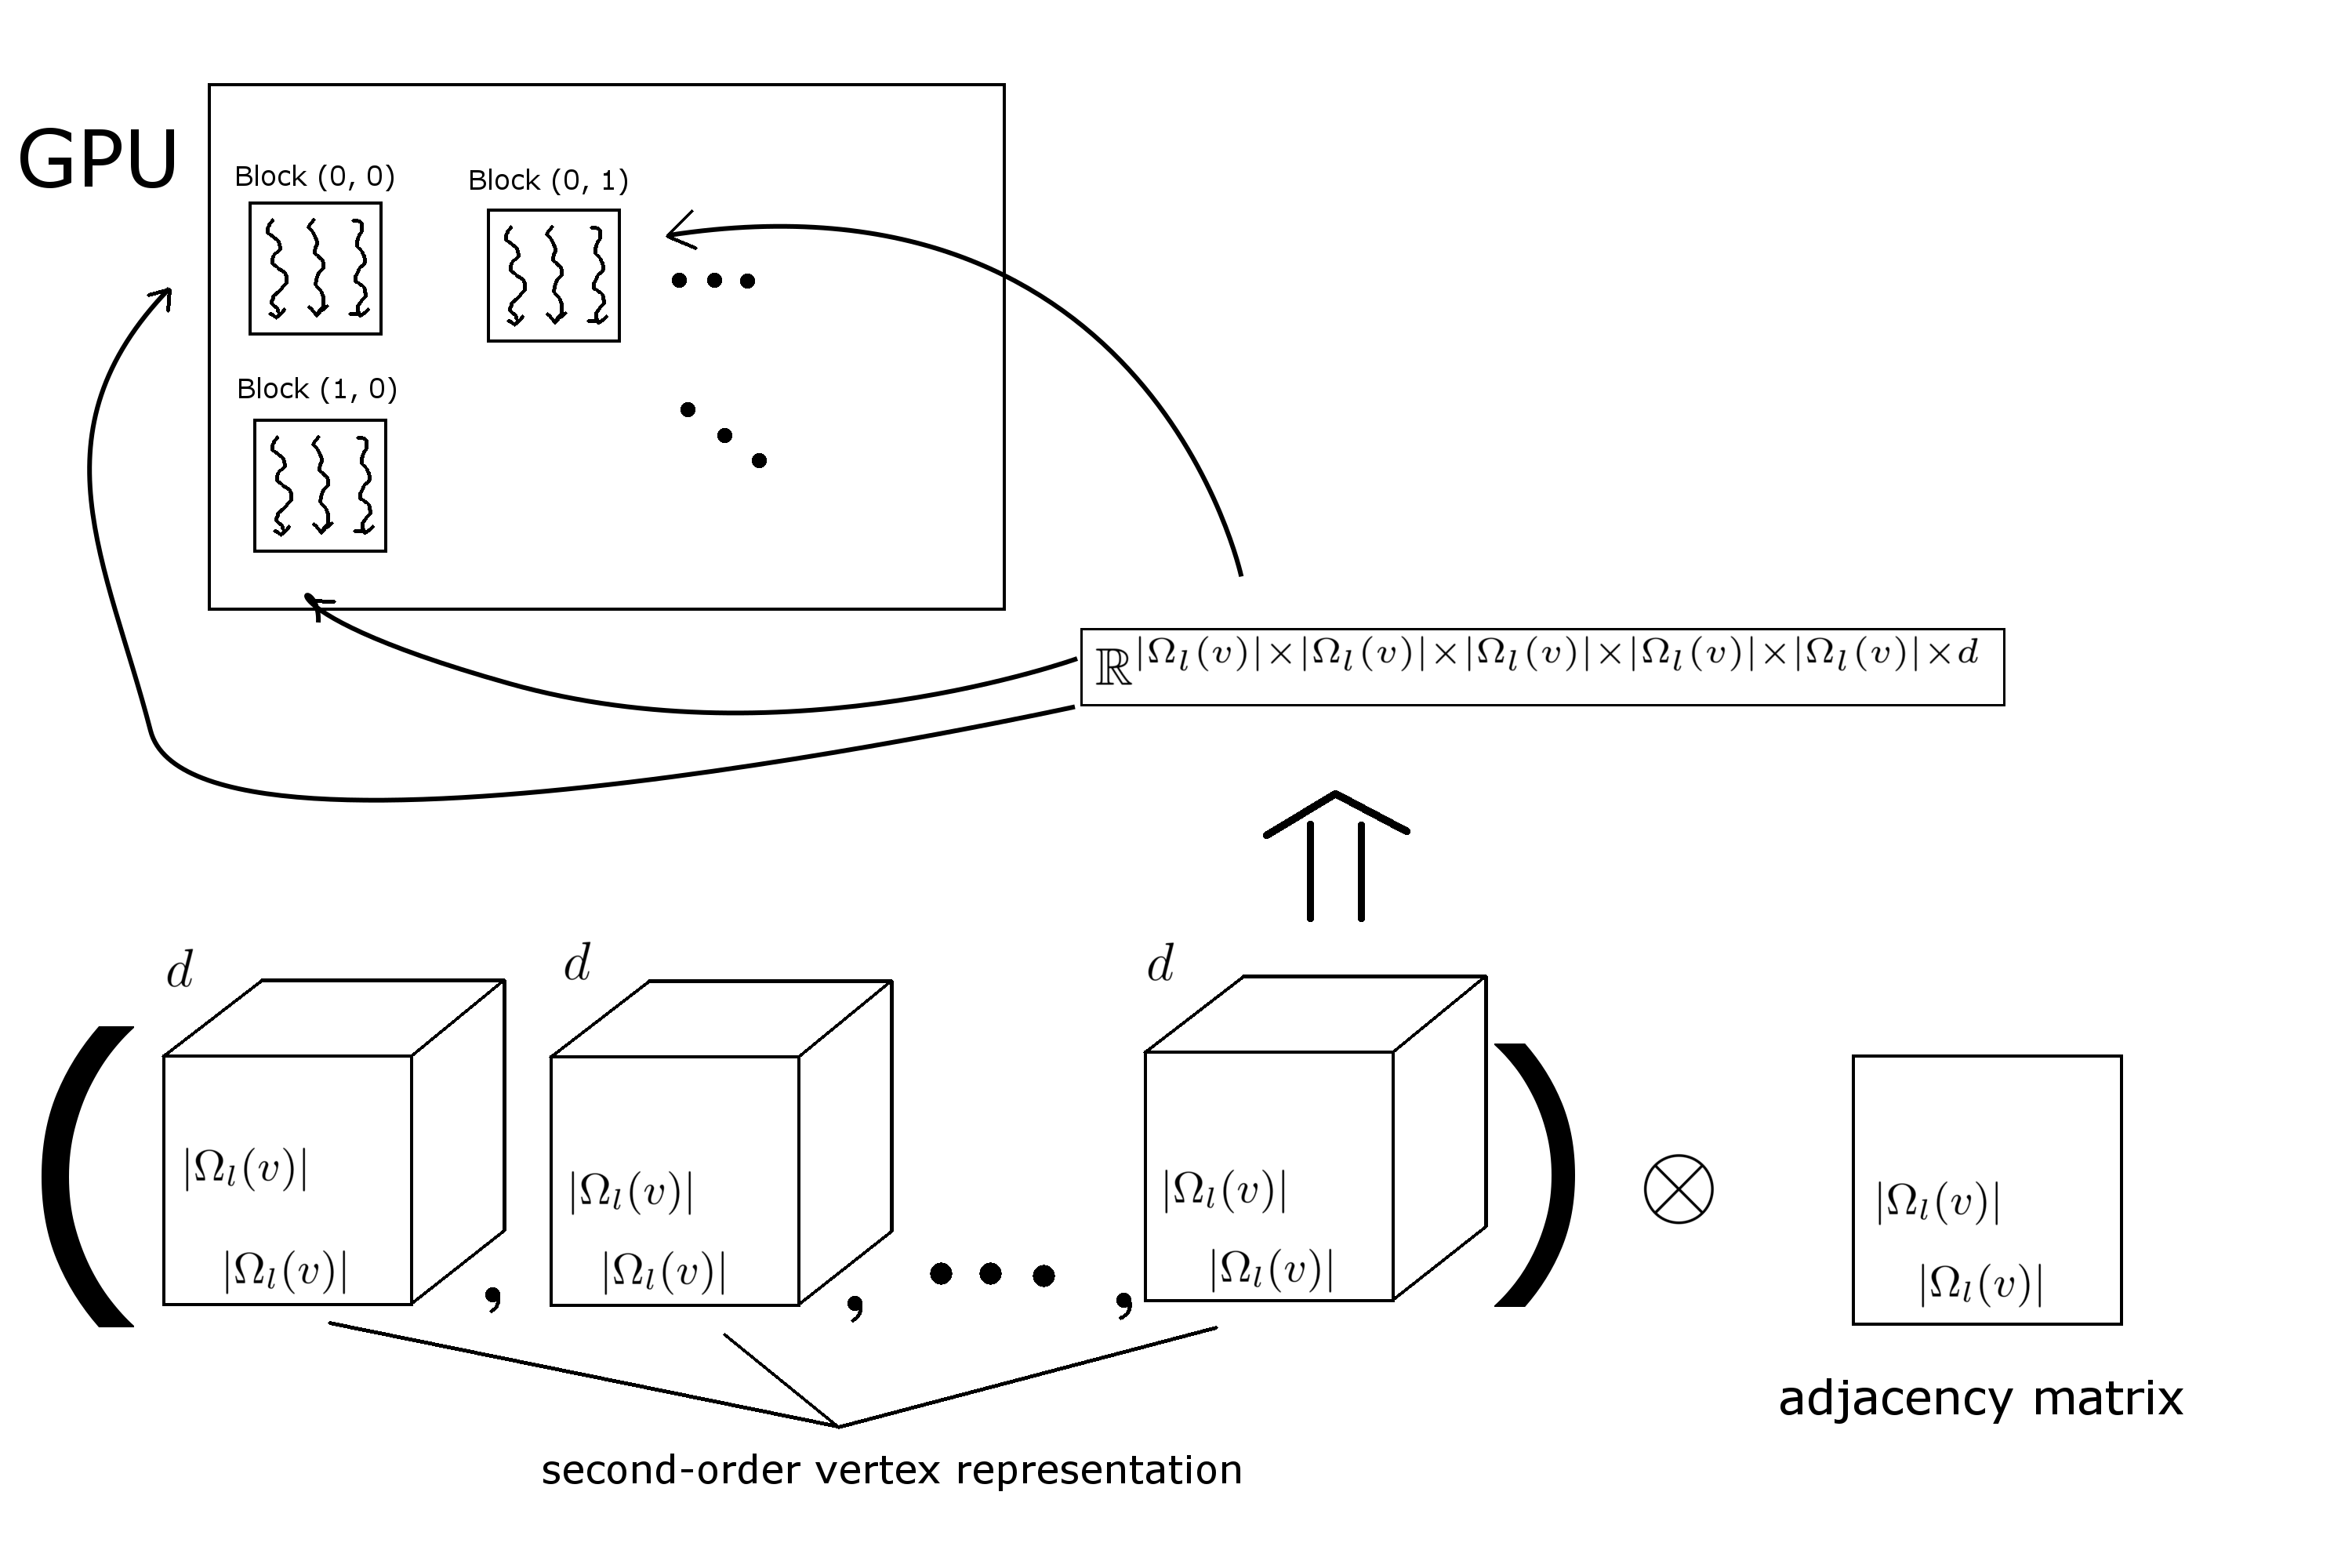
\includegraphics[width=\columnwidth]{GPU_multithreading.png}
\end{figure}


Again, synchronization is also a real challenge: all the updating operations must be atomic. However, having too many atomic operations can slow down our concurrent algorithm. That is why we have to design our GPU algorithm with the minimum possible number of atomic operations. We obtain a much better performance with GPU after careful consideration of all factors.

\subsubsection{CPU Multi-threading in Gradient Computation}

Given a minibatch of $M$ training examples, it is a natural idea to separate the gradient computation jobs into multiple threads such that each thread processes exactly one training example at a time before processing the next example. We must make sure that there is no overlap among these threads. After completing the gradient computations from all these $M$ training examples, we sum up all gradients, average them by $M$, and apply a variant of Stochastic Gradient Descent to optimize the neural networks before moving to the next minibatch. \\ \\
Technically, suppose that we can execute $T$ threads concurrent at a time for gradient computation jobs. Before every training starts, we initialize exactly $T$ identical dynamic computation graphs by GraphFlow. Given a minibatch of $M$ training examples, we distribute the examples to $T$ threads, each thread uses a different dynamic computation graph for its gradient computation job. By this method, there is absolutely no overlap and our training is completely synchronous. \\ \\
The minibatch training with CPU multi-threading is described by Figure~\ref{fig:CPU_multithreading}: 

\begin{figure}[h]
\caption{CPU multi-threading for gradient computation}
\label{fig:CPU_multithreading}
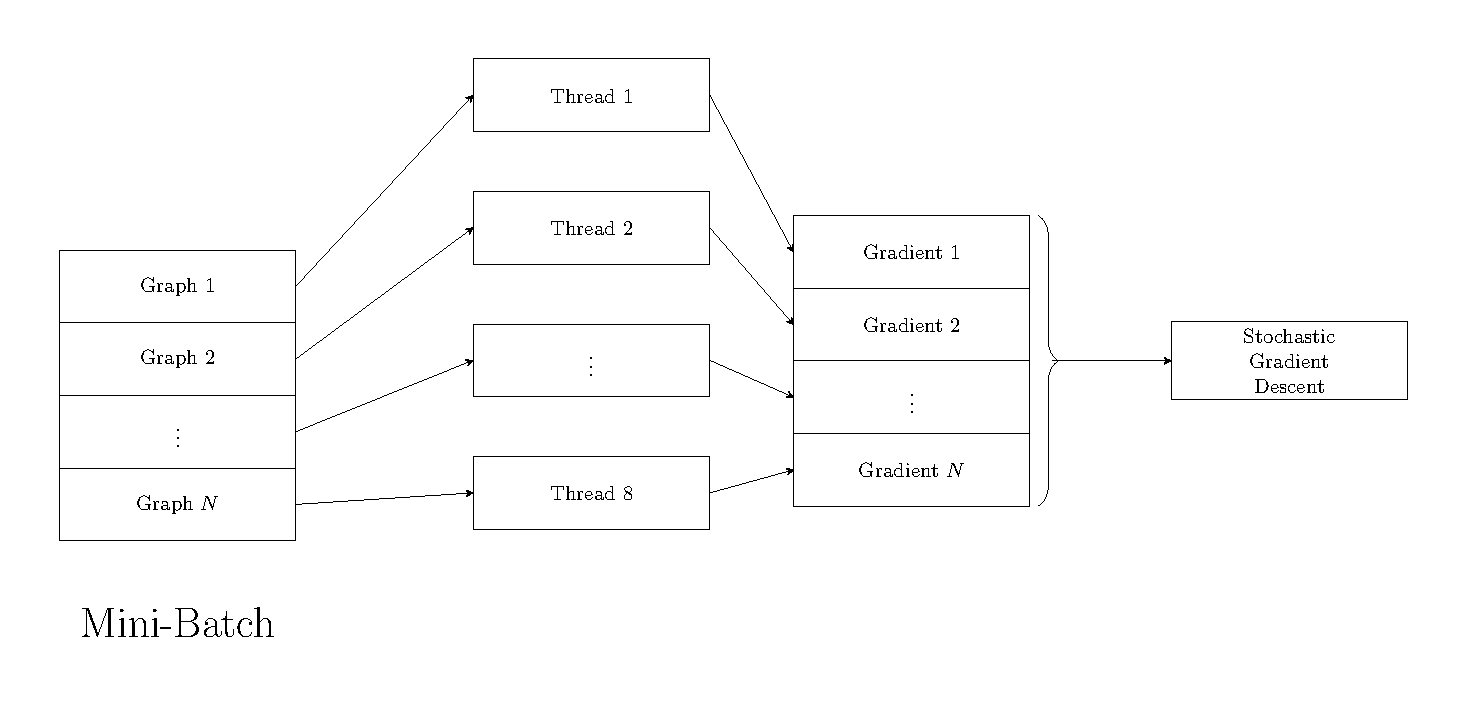
\includegraphics[width=\columnwidth]{CPU_box_flow}
\end{figure}

\section{Experiments and Results}

\subsection{Matrix Multiplication}

To demonstrate the efficiency of our GPU matrix multiplication, we establish several performance tests and measure the running time against an $O(N^3)$ CPU matrix multiplication. The sizes of the test matrices are $N \in \{128, 256, 512, 1024\}$. In the largest case, we observe that GPU gives a factor of 200x improvement. Table~\ref{tab:matrix_mult} gives the details.

\begin{table}[h]
\begin{tabular}{||c | c | c | c | c ||}
	\hline
	Method & N = 128 & N = 256 & N = 512 & N = 1024 \\
	\hline\hline
	CPU & 22 ms & 379 ms & 2,274 ms & 15,932 ms \\
	\hline
	GPU & $<$ 1 ms & 4 ms & 15 ms & 70 ms \\
	\hline
\end{tabular}
\caption{GPU vs CPU matrix multiplication}\label{tab:matrix_mult}
\end{table}

\begin{figure}[h]
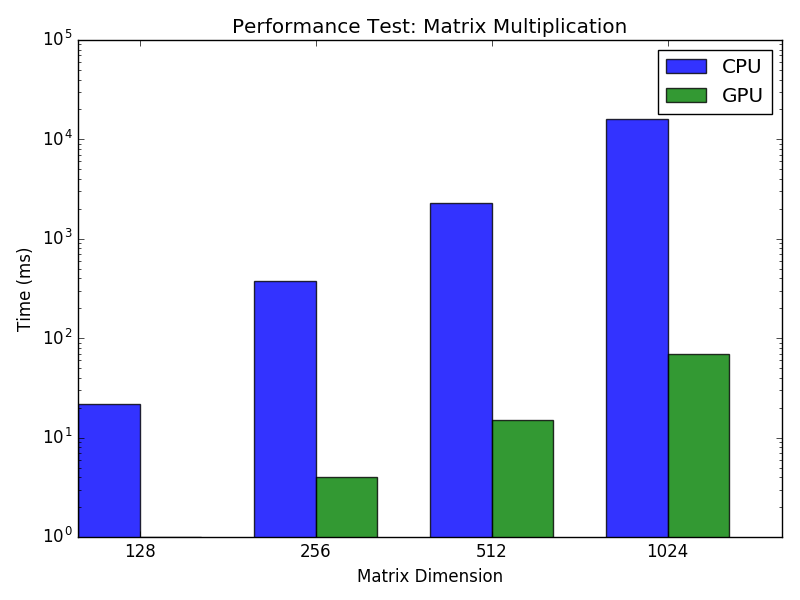
\includegraphics[width=\columnwidth]{Matrix_Multiplication}
\caption{GPU vs CPU matrix multiplication running time (milliseconds) in $\log_{10}$ scale}
\label{fig:matrix_mult}
\end{figure}

\subsection{Tensor Contraction}

We also compare the GPU implementation of tensor contraction with the CPU implementation. We must remark that the complexity of tensor contraction is $O(18 \times |\Omega_l(v)|^5 \times d)$, which grows exponentially with the size of receptive field $|\Omega_l(v)|$ and grows linearly with the number of channels. We have a constant 18 as the number of unique contractions in the second-order case. We have several tests with the size of the receptive field $|\Omega_l(v)|$ ranging across $\{5, 10, 20, 35\}$ and the number of channels $d$ ranging across $\{10, 20\}$. In the largest case with $|\Omega_l(v)| = 35$ and $d = 20$, we observe that GPU gives a factor of approximately 62x speedup. Table~\ref{tab:tensor_contraction} gives the details.
  
\begin{table}
\caption{GPU and CPU tensor contraction}\label{tab:tensor_contraction}
\begin{tabular}{|| c | c | c | c | c ||}
	\hline
	$|\Omega_l(v)|$ & $d$ & Floating-points & CPU & GPU \\
	\hline\hline
	5 & 10 & 562,500 & 3 ms & 3 ms \\
	\hline
	5 & 20 & 1,125,000 & 7 ms & 1 ms \\
	\hline
	10 & 10 & 18,000,000 & 56 ms & 1 ms \\
	\hline
	10 & 20 & 36,000,000 & 103 ms & 3 ms \\
	\hline
	20 & 10 & 576,000,000 & 977 ms & 18 ms \\
	\hline 
	20 & 20 & 1,152,000,000 & 2,048 ms & 27 ms \\
	\hline
	35 & 10 & 9,453,937,500 & 12,153 ms & 267 ms \\
	\hline
	35 & 20 & 18,907,875,000 & 25,949 ms & 419 ms \\
	\hline
\end{tabular}
\end{table}

\begin{figure}
\caption{GPU vs CPU tensor contraction running time (milliseconds) in $\log_{10}$ scale}\label{fig:tensor_contraction}
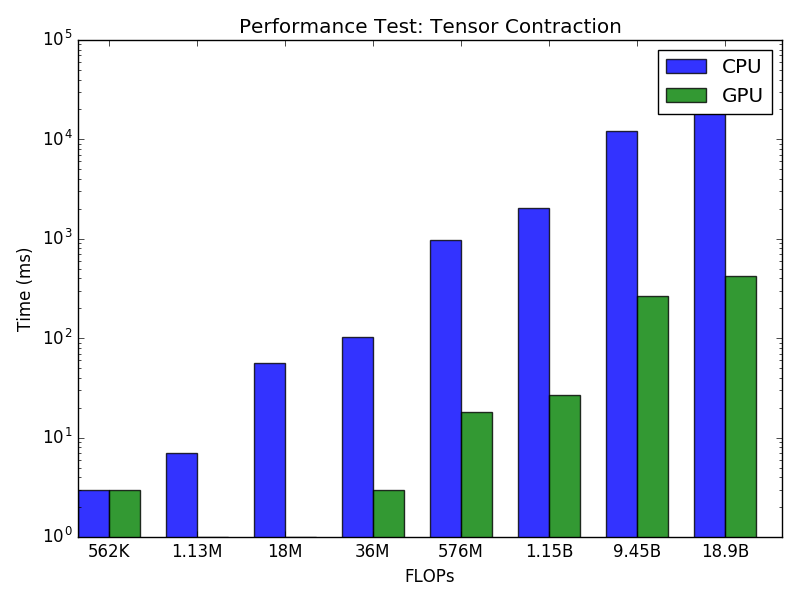
\includegraphics[width=\columnwidth]{Tensor_Contraction}
\end{figure} 


\subsection{Putting all operations together}

In this experiment, we generate synthetic random input graphs by the Erdos-Renyi $p = 0.5$ model. The number of vertices $|V|$ ranges across $\{10, 15, 20, 25\}$. We fix the maximum size of the receptive field $|\Omega_l(v)|$ as 10 and 15, the number of channels $d$ as 10, and the number of layers of the neural network $L$ as 6. In the largest case of the graph with 25 vertices, GPU gives a factor of approximately 6x speedup. Table~\ref{tab:erdos_renyi} gives the details. 

\begin{table}[h]
\caption{GPU and CPU network evaluation}\label{tab:erdos_renyi}
\begin{tabular}{|| c | c | c | c | c | c ||}
	\hline
	$|V|$ & Max $|\Omega_l(v)|$ & $d$ & $L$ & CPU & GPU \\
	\hline\hline
	10 & 10 & 10 & 6 & 1,560 ms & 567 ms \\
	\hline
	15 & 10 & 10 & 6 & 1,664 ms & 543 ms \\
	\hline 
	20 & 15 & 10 & 6 & 7,684 ms & 1,529 ms \\
	\hline
	25 & 15 & 10 & 6 & 11,777 ms & 1,939 ms \\
	\hline
\end{tabular}
\end{table}

\subsection{Small Molecular Dataset}

This is the total training and testing time on a small dataset of 4 molecules $CH_4$, $NH_3$, $H_20$, $C_2H_4$ with 1,024 epochs. After each epoch, we evaluate the neural network immediately. CCN 1D denotes the Covariant Compositional Networks with the first-order representation and the number of layers ranging across $\{1, 2, 4, 8, 16\}$. CCN 2D denotes the Covariant Compositional Networks using a second-order representation and the number of layers ranging across $\{1, 2\}$. The number of channels is $d = 10$ in all settings. In this experiment, we use 4 threads for the training minibatches of 4 molecules and compare the running time with the single thread case. All models are fully converged.

\begin{table}[h]
\caption{Single thread vs Multiple threads}\label{tab:basic_molecules}
\begin{tabular}{|| c | c | c | c ||}	
	\hline
	Model & Layers & Single-thread & Multi-thread \\
	\hline\hline
	CCN 1D & 1 & 1,836 ms & 874 ms \\
	\hline
	CCN 1D & 2 & 4,142 ms & 1,656 ms\\
	\hline
	CCN 1D & 4 & 9,574 ms & 3,662 ms \\
	\hline
	CCN 1D & 8 (deep) & 20,581 ms & 7,628 ms \\
	\hline
	CCN 1D & 16 (very deep) & 42,532 ms & 15,741 ms\\
	\hline
	CCN 2D & 1 & 35 seconds & 10 seconds \\
	\hline
	CCN 2D & 2 & 161 seconds & 49 seconds \\
	\hline
\end{tabular}
\end{table}

\subsection{HCEP Dataset}

The Harvard Clean Energy Project (HCEP) dataset \cite{Johannes} contains 2.3 million molecules that are potential future solar energy materials. By the computationally expensive Density Functional Theory (which should be less computationally expensive once efficient quantum computers hit the market), the authors of HCEP computed the Power Conversion Energy (PCE) for each molecule. PCE values are continuous ranging from 0 to 11. For our experiments, we extract 50,000 molecules and allocate 30,000 molecules for training, 10,000 molecules for validation, and 10,000 molecules for testing. Each molecule is given by a SMILES code. We transform the SMILES codes into adjacancy matrices where each atom is a vertex and the atom type is the input vertex label. \\ \\
When using the Dictionary Weisfeiler-Lehman graph kernel, we investigated the number of non-isomorphic receptive fields across this dataset. In the set of 50,000 molecules that we selected, there are in total 11,172 different receptive fields of level 3. This number is very manageable as the size of the dictionary. We also applied \textit{sparse} Support Vector Regression to these sparse feature vectors and obtained good results.

\subsubsection{Visualization}

For the purpose of visualization, we rounded PCE values to the nearest integer. We applied Principal Component Analysis (PCA) and t-Distributed Stochastic Neighbor Embedding (t-SNE) \cite{Maaten} on the feature vectors produced by both Weisfeiler-Lehman (WL) graph kernel and our Covariant Compositional Networks.

\begin{figure}[h]
\caption{WL feature vectors with PCA and t-SNE}\label{fig:WL_features}
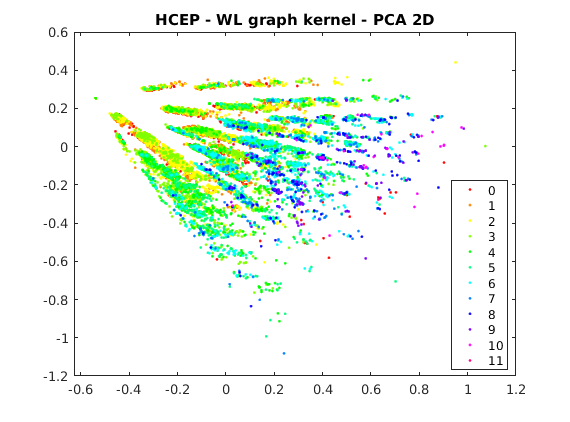
\includegraphics[width=0.49\columnwidth]{PCA_WL}
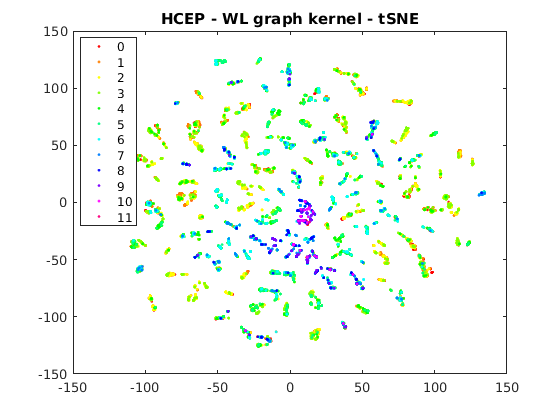
\includegraphics[width=0.49\columnwidth]{tSNE_WL}
\end{figure}

\begin{figure}[h]
\caption{CCN 1D feature vectors with PCA and t-SNE}\label{fig:CCN_1D_features}
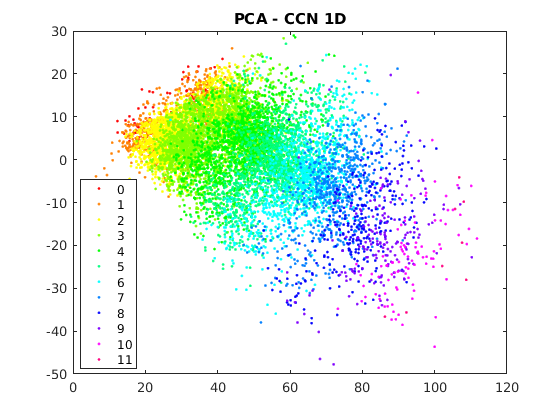
\includegraphics[width=0.49\columnwidth]{PCA_CCN_1D}
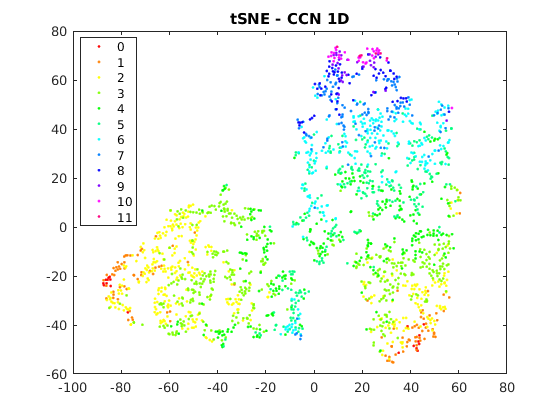
\includegraphics[width=0.49\columnwidth]{tSNE_CCN_1D}
\end{figure}

\begin{figure}[h]
\caption{CCN 2D feature vectors with PCA and t-SNE}\label{fig:CCN_2D_features}
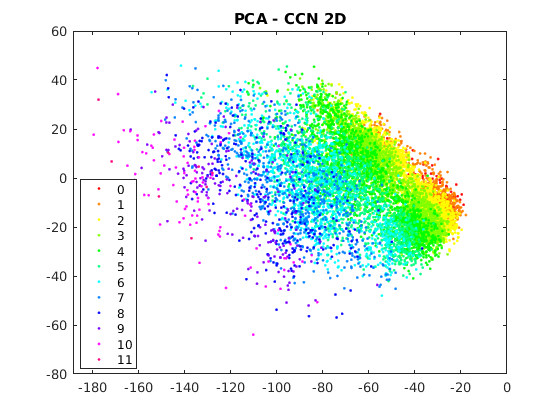
\includegraphics[width=0.49\columnwidth]{PCA_CCN_2D}
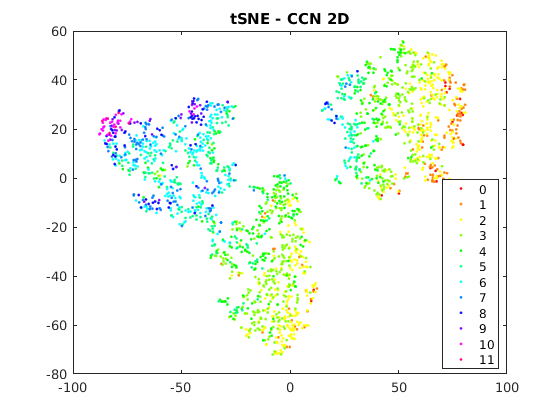
\includegraphics[width=0.49\columnwidth]{tSNE_CCN_2D}
\end{figure}
We observe that our CCN models give a much better visualization in the 2-dimensional visualization. We can see the separations among the clusters where each cluster is associated with a (rounded integer) PCE value.

\subsubsection{Regression tasks}

Using the Weisfeiler-Lehman (WL) graph kernel, we apply Linear regression, Gaussian Process and SVM for the task of regressing PCE values. We find the optimal hyperparameters in the validation set. For linear regression, the regularization parameter $C \in \{0, 10^{-4}, 10^{-3}, 10^{-2}, 10^{-1}, 1, 10, 100\}$. For Gaussian Process, we choose a Radial Basis Function (RBF) kernel with the optimal $\sigma = 2$, with the noise parameter selected from the range from $0$ to $100$. For SVM, the RBF kernel is chosen with $\sigma = 0.01$, and regualarization parameter $C = 100$. \\ \\
Regarding training our Covariant Compositional Networks, for the first-order representation (CCN 1D), we selected the best architecture among setups with the number of layers as 1, 2, 3, 4, 5, 6, and 7. CCN 1D gives the best result with 7 levels. For the second-order representation (CCN 2D), the number of layers is 1 and 2. CCN 2D gives the best result with a single level. The number of channels is fixed as 10. We employ Stochastic Gradient Descent with Adam optimization. The learning rate is initially $10^{-3}$ and linearly decayed to $10^{-6}$ in $10^6$ iterations. The batch size is fixed as 64. The maximum number of epochs is 1024 in all settings. \\ \\
We also compare with two other state-of-the-art graph neural networks: Neural Graph Fingerprint (NGF) and Learning Convolutional Neural Networks (LCNN). NGF has the maximum of 3 levels and the number of hidden states is 10. LCNN has 2 convolutional layers. In all graph neural networks settings, we always have a linear regression on top of the network. \\ \\
We estimate the performance of our models in both Mean Average Error (MAE) and Root Mean Square Error (RMSE). In both metrics, Covariant Compositional Networks outperform Weisfeiler-Lehman graph kernel, Neural Graph Fingerprint and Learning Convolutional Neural Networks. We observe that training for higher-order representations is increasingly more difficult since the size of the representation grows exponentially. Some techniques have been used to solve this problem, for example thresholding the maximum size of receptive fields. More training is probably required to obtain the full potential of higher-order representations.

\begin{table}[h]
\caption{HCEP dataset}\label{tab:HCEP}
\begin{tabular}{|| c | c | c ||} 
\hline
Model & Test MAE & Test RMSE \\
\hline
\hline
WL + Linear Regression & 0.805 & 1.096 \\
\hline
WL + Gaussian Process & 0.760 & 1.093 \\ 
\hline
WL + Support Vector Machine & 0.878 & 1.202 \\
\hline
NGF & 0.851 & 1.177 \\
\hline
LCNN & 0.718 & 0.973 \\
\hline 
CCN 1D & {\color{red} 0.216} & {\color{red} 0.291} \\
\hline
CCN 2D & {\color{red} 0.340} & {\color{red} 0.449} \\
\hline
\end{tabular}
\end{table}

\begin{figure}[h]
\caption{Testing errors vs Number of training epochs. Top: MAE. Bottom: RMSE}\label{fig:error_vs_epoch}
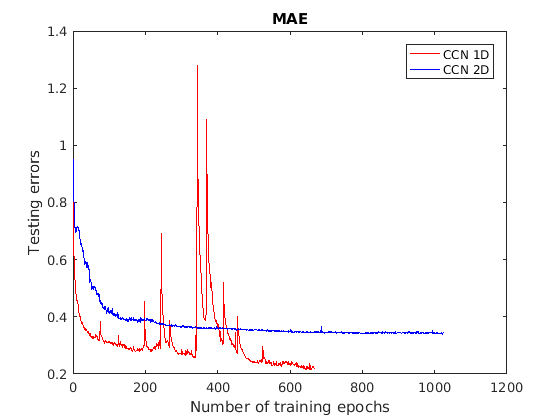
\includegraphics[width=\columnwidth]{MAE}
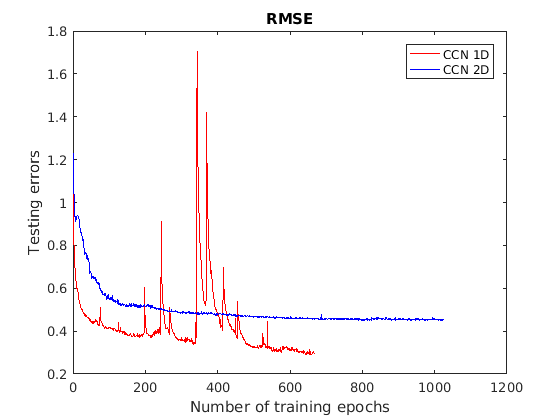
\includegraphics[width=\columnwidth]{RMSE}
\end{figure}

\begin{figure}[h]
\caption{Distributions of the predicted PCE values and the expected PCE values. Top: CCN 1D. Bottom: CCN 2D}\label{fig:predict_vs_actual}
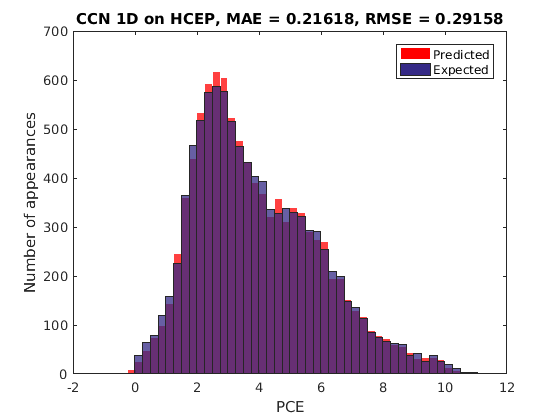
\includegraphics[width=\columnwidth]{Result_CCN_1D}
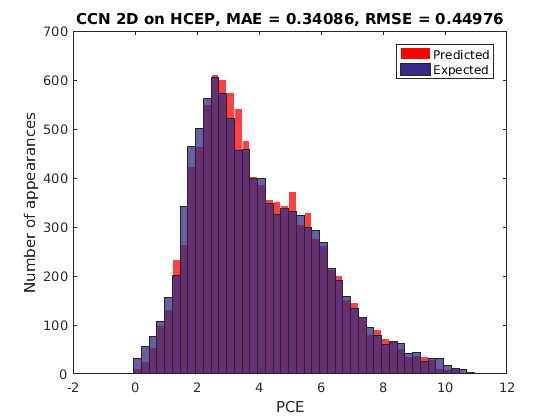
\includegraphics[width=\columnwidth]{Result_CCN_2D}
\end{figure}

\section{Conclusion and Future Research}

We extended the state-of-the-art Weisfeiler-Lehman graph kernel and generalized convolution operation for Covariant Compositional Networks using higher-order representations. We obtained very promising results and outperformed two other current state-of-the-art graph neural networks, Neural Graph Fingerprint and Learning Convolutional Neural Networks, on a subset the Harvard Clean Energy Project dataset. Thanks to parallelization, we significantly improved our empirical results. \\ \\
We are developing our custom Deep Learning framework in C++, \textbf{GraphFlow}, which supports automatic and symbolic differentitation, dynamic computation graph as well as complex tensor / matrix operations in CUDA with GPU computation acceleration. We expect that this framework will enable us to design more flexible, efficient graph neural networks with molecular applications at a large scale in the future.

\section{Acknowledgements}

We would like to acknowledge Professor Risi Kondor for his valuable instruction and especially for his ideas for generalizing convolution operations in graphs. We also want to thank other members of Machine Learning group at the University of Chicago for their dedicated support. \\ \\
Some of the neural network training in this paper was done using the Techstaff cluster of the Department of Computer Science and Midway cluster of the UChicago Computing Research Center.

\bibliographystyle{IEEEtran}

\bibliography{mybib}

\begin{thebibliography}{9}

\bibitem[1]{Nino}
   N. Shervashidze, P. Schweitzer, E. J. van Leeuwen, K. Mehlhorn, K. M. Borgwardt,
   ``Weisfeiler-Lehman Graph Kernels'',
   \textit{Journal of Machine Learning Research}, vol.~12, 2011.
   
\bibitem[2]{Johannes}
   J. Hachmann, R. O. Amaya, S. A. Evrenk, C. A. Bedolla, R. S. S. Carrera, A. G. Parker, L. Vogt, A. M. Brockway, and A. A. Guzik,
   ``The Harvard Clean Energy Project: Large-Scale Computational Screening and Design of Organic Photovoltaics on the World Community Grid'',
   \textit{The Journal of Physical Chemistry Letters}, pp.~2241--2251, 2011.

\bibitem[3]{Risi}
   R. I. Kondor, and J. Lafferty,
   ``Diffusion Kernels on Graphs and Other Discrete Structures'',
   \textit{International Conference on Machine Learning (ICML)}, 2002.
   
\bibitem[4]{Nils}
   N. M. Kriege, P. L. Giscard, R. C. Wilson,
   ``On Valid Optimal Assignment Kernels and Applications to Graph Classification'',
   \textit{Neural Information Processing Systems (NIPS)}, 2016.

\bibitem[5]{Steven}
   S. Kearnes, K. McCloskey, M. Berndl, V. Pande, P. Riley,
   ``Molecular Graph Convolutions: Moving Beyond Fingerprints'',
   \textit{Journal of Computer-Aided Molecular Design}, vol.~30, pp.~595--608, 2016.

\bibitem[6]{Duvenaud}
   D. Duvenaud, D. Maclaurin, J. A. Iparraguirre, R. G. Bombarelli, T. Hirzel, A. A. Guzik, R. P. Adams,
   ``Convolutional Networks on Graphs for Learning Molecular Fingerprints'',
   \textit{Neural Information Processing Systems (NIPS)}, 2015.
   
\bibitem[7]{Thomas}
   T. N. Kipf, M. Welling,
   ``Semi-Supervised Classification with Graph Convolutional Networks'',
   \textit{International Conference on Learning Representations (ICLR)}, 2017.

\bibitem[8]{Maaten}
   L. V. D. Maaten, G. Hinton,
   ``Visualizing Data using t-SNE'',
   \textit{Journal of Machine Learning Research}, vol.~9, pp.~2579--2605, 2008.
   
\bibitem[9]{Niepert}
   M. Niepert, M. Ahmed, K. Kutzkov,
   ``Learning Convolutional Neural Networks'',
   \textit{International Conference on Machine Learning (ICML)}, 2016.
   
\bibitem[10]{Hochreiter}
   S. Hochreiter, J. Schmidhuber,
   ``Long Short-Term Memory'',
   \textit{Neural Computation}, 1997.

\bibitem[11]{Chung}
   J. Chung, C. Gulcehre, K. Cho, Y. Bengio,
   ``Empirical Evaluation of Gated Recurrent Neural Networks on Sequence Modeling'',
   \textit{Neural Information Processing Systems (NIPS) Workshop}, 2014.
   
\bibitem[11]{Li}
   Y. Li, D. Tarlow, M. Brockschmidt, R. Zemel,
   ``Gated Graph Sequence Neural Networks'',
   \textit{International Conference of Learning Representations (ICLR)}, 2016.

\bibitem[12]{Google-Research}
   M. Abadi, A. Agarwal, P. Barham, E. Brevdo, Z. Chen, C. Citro, G. S. Corrado, A. Davis, J. Dean, M. Devin, S. Ghemawat, I. Goodfellow, A. Harp, G. Irving, M. Isard, Y. Jia, R. Jozefowicz, L. Kaiser, M. Kudlur, J. Levenberg, D. Mane, R. Monga, S. Moore, D. Murray, C. Olah, M. Schuster, J. Shlens, B. Steiner, I. Sutskever, K. Talwar, P. Tucker, V. Vanhoucke, V. Vasudevan, F. Viegas, O. Vinyals, P. Warden, M. Wattenberg, M. Wicke, Y. Yu, X. Zheng,
   ``TensorFlow: Large-Scale Machine Learning on Heterogeneous Distributed Systems'',
   \textit{https://arxiv.org/abs/1603.04467}, 2016.

\bibitem[13]{PyTorch}
   A. Paszke, S. Gross, S. Chintala, G. Chanan, E. Yang, Z. DeVito, Z. Lin, A. Desmaison, L. Antiga, A. Lerer,
   ``Automatic differentiation in PyTorch'',
   \textit{Neural Information Processing Systems (NIPS)}, 2017.

\bibitem[14]{Theano}
    R. Al-Rfou, G. Alain, A. Almahairi, C. Angermueller, D. Bahdanau, N. Ballas, F. Bastien, J. Bayer, A. Belikov, A. Belopolsky, Y. Bengio, A. Bergeron, J. Bergstra, V. Bisson, J. B. Snyder, N. Bouchard, N. Boulanger-Lewandowski, X. Bouthillier, A. de Brébisson, O. Breuleux, P. Carrier, K. Cho, J. Chorowski, P. Christiano, T. Cooijmans, M. Cote, M. Cote, A. Courville, Y. N. Dauphin, O. Delalleau, J. Demouth, G. Desjardins, S. Dieleman, L. Dinh, M. Ducoffe, V. Dumoulin, S. E. Kahou, D. Erhan, Z. Fan, O. Firat, M. Germain, X. Glorot,
   ``Theano: A Python framework for fast computation of mathematical expressions'',
   \textit{https://arxiv.org/abs/1605.02688}, 2016.
   
\bibitem[15]{Mxnet}
    T. Chen, M. Li, Y. Li, M. Lin, N. Wang, M. Wang, T. Xiao, B. Xu, C. Zhang, Z. Zhang,
   ``MXNet: A Flexible and Efficient Machine Learning Library for Heterogeneous Distributed Systems'',
   \textit{Neural Information Processing Systems (NIPS) Workshop}, 2016.
   
\bibitem[16]{TF-fold}
    M. Looks, M. Herreshoff, D. Hutchins, P. Norvig,
   ``Deep Learning with Dynamic Computation Graphs'',
   \textit{International Conference of Learning Representations (ICLR)}, 2017.

\end{thebibliography}

\clearpage

\section{Appendix}

\begin{center}
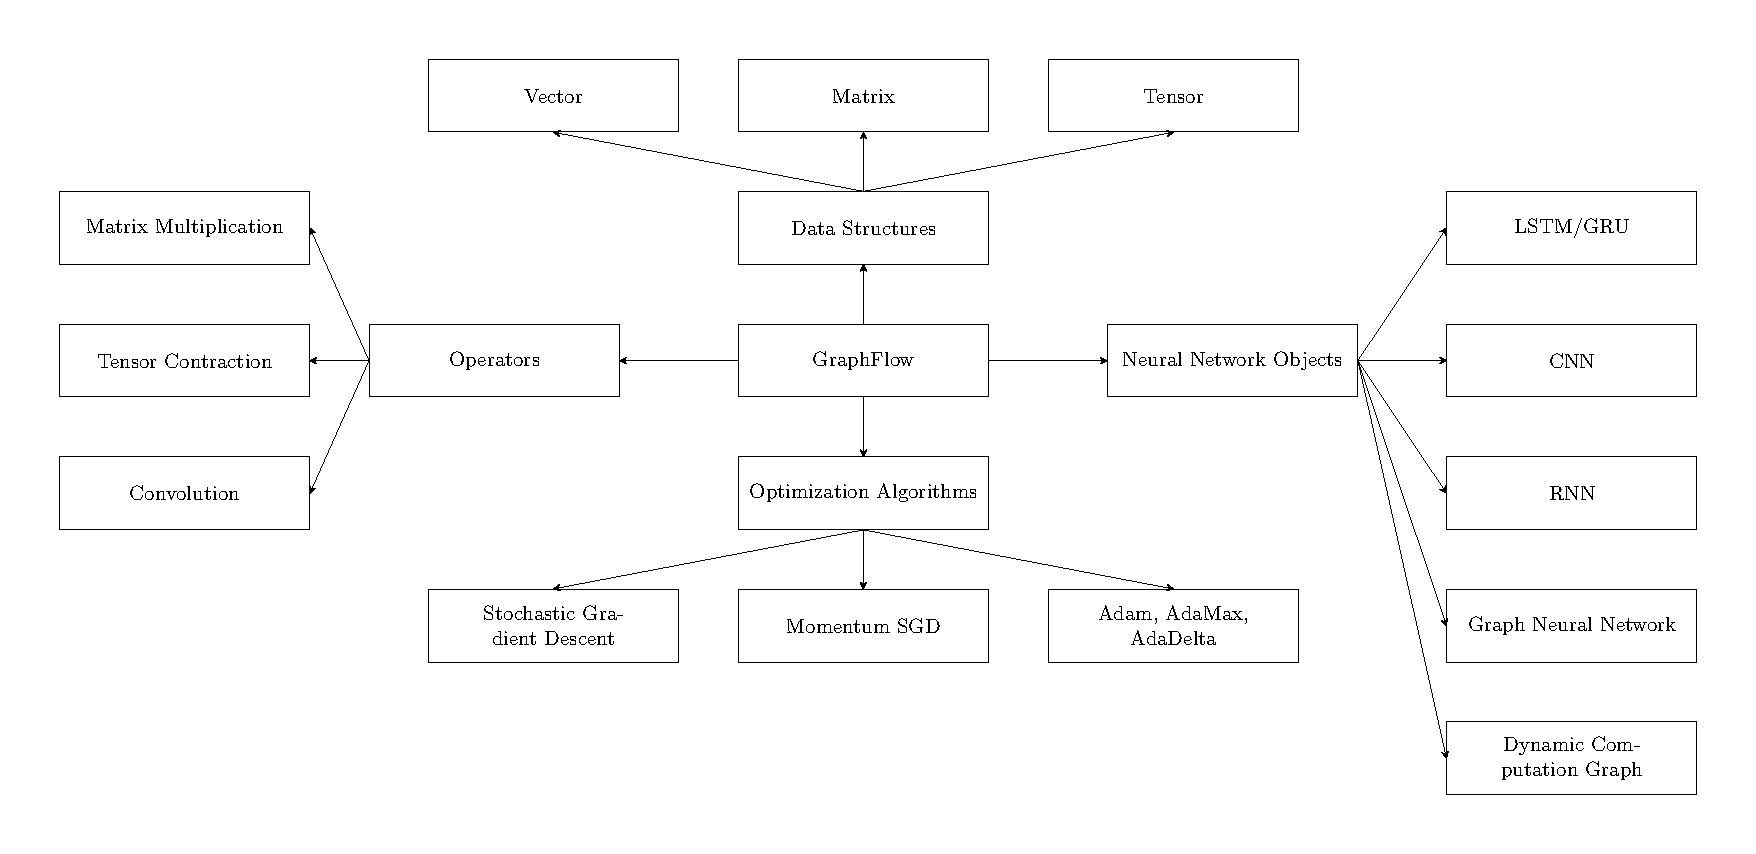
\includegraphics[scale=0.56]{GraphFlow_box_flow}
\end{center}

% \begin{thebibliography}{9}
% \bibitem[1]{Davis80-COP}
%   S.\ B.\ Davis and P.\ Mermelstein,
%   ``Comparison of parametric representation for monosyllabic word recognition in continuously spoken sentences,''
%   \textit{IEEE Transactions on Acoustics, Speech and Signal Processing}, vol.~28, no.~4, pp.~357--366, 1980.
% \bibitem[2]{Rabiner89-ATO}
%   L.\ R.\ Rabiner,
%   ``A tutorial on hidden Markov models and selected applications in speech recognition,''
%   \textit{Proceedings of the IEEE}, vol.~77, no.~2, pp.~257-286, 1989.
% \bibitem[3]{Hastie09-TEO}
%   T.\ Hastie, R.\ Tibshirani, and J.\ Friedman,
%   \textit{The Elements of Statistical Learning -- Data Mining, Inference, and Prediction}.
%   New York: Springer, 2009.
% \bibitem[4]{YourName17-XXX}
%   F.\ Lastname1, F.\ Lastname2, and F.\ Lastname3,
%   ``Title of your INTERSPEECH 2017 publication,''
%   in \textit{Interspeech 2017 -- 18\textsuperscript{th} Annual Conference of the International Speech Communication Association, August 20?24, Stockholm, Sweden, Proceedings, Proceedings}, 2017, pp.~100--104.
% \end{thebibliography}

\end{document}
